\section{Decision and implementation}

\subsection{Decision}
For the first prototype implementation, the combination of MATSim and SUMO was chosen in order to leverage the strengths of both tools. MATSim offers scalable, agent-based demand generation, allowing realistic daily schedules and routes to be implemented based on activity patterns and POIs. SUMO, on the other hand, is a high-performance microscopic traffic simulator that can accurately map vehicle movements.

By combining both tools, the generation of agents and routes (MATSim) and the actual simulation (SUMO) are separated. In addition, SUMO can be controlled by TraCI during runtime. This creates a modular and scalable system architecture that effectively represents electric mobility scenarios.

Other approaches described, such as BEAM and SAGA, were initially rejected. BEAM proved impractical due to the high complexity of the feedback loop caused by replanning and the large overhead. Although SAGA offers a very promising pipeline and was also tested, it was also ruled out due its insufficient documentation and flawed error handling at the the time of the project.

\subsection{Implementation}
The following section describes the first prototypical workflow and the transition to the current implementation. Initially, agent-based daily schedules and travel routes were generated in MATSim, while microscopic traffic simulation was subsequently performed in SUMO.
However, during development and especially during stress testing, this approach proved to be error-prone: There were repeated problems converting MATSim networks and routes into SUMO-compatible formats, which meant that simulations could not be run with the generated data.

These difficulties ultimately led to a switch to the current workflow, in which the routes are now generated entirely by our own Python scripts independently of MATSim.

\subsubsection{Prototyping}
The project's initial design and vision were promising because the tools offer powerful options for creating simulations. Coupling MATSim's demand generation with SUMO's microscopic simulation created a modular, flexible workflow well-suited for electric mobility scenarios at large and detailed scales.


\begin{figure}[ht]
    \centering
    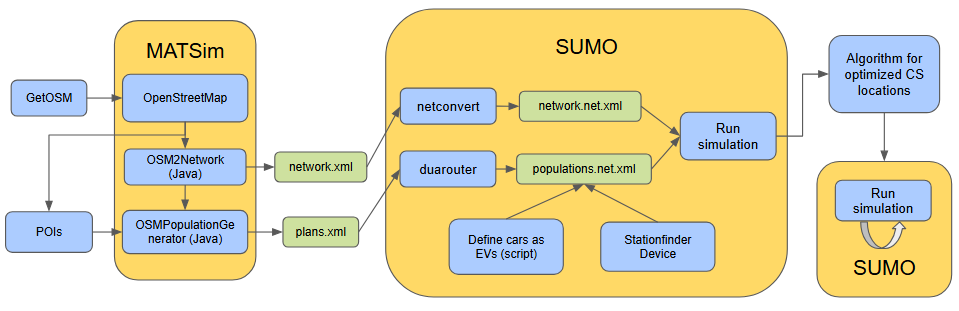
\includegraphics[width=\textwidth]{images/Bild_MATSim_SUMO.png}
    \caption{Flowchart of Prototype Design}
    \label{fig:oldDesign}
\end{figure}

The figure above illustrates the structure of the initial workflow. A built-in integration of SUMO's \texttt{osmGet} script retrieves raw OSM data, although alternative tools like JOSM could be used as well. This data is then converted by two developed MATSim functions into a \texttt{network.xml} file, along with a \texttt{plans.xml} file generated from the provided points of interests (POIs). The \texttt{plans.xml} contains the travel routes agents will follow between their POIs.

Next, the system converts these files into SUMO-compatible formats using \texttt{netconvert} and \texttt{duarouter}, which process the network's nodes and edges. After successful conversion, all vehicles defined in the \texttt{population.net.xml} file are overwritten as electric vehicles (EVs) and equipped with a \texttt{stationfinder} device. This device allows them to dynamically reroute to nearby charging stations if needed, deviating from their original paths.

The simulation is then executed, and an optimization algorithm analyzes the logged results to improve the placement of charging stations. The updated station locations serve as input for the next iteration - forming a optimization loop that refines the infrastructure with each cycle.

The placement and optimization of charging stations has not yet been implemented in this prototype workflow, as the conversion from MATSim to SUMO already led to errors.

\subsubsection{Refactoring and technical learning}
As described above, the combination of MATSim and SUMO proved to be too error-prone to continue. This resulted in a refactoring of the project, during which previously developed Java classes and dependencies were removed. This step significantly reduced complexity, as the Java-based structure had introduced overhead and rigidity.

Despite its limitations, the initial prototype workflow was instrumental in building a deeper understanding of SUMO's simulation architecture, including the required input files, data formats and configuration files. This foundation greatly accelerated the development of the further implementations.

\subsubsection{Current implementation}
The current implementation builds on the experience gained with the first prototype, but completely replaces MATSim. Demand generation is now performed by proprietary scripts in pre-processing and flows directly into the subsequent optimization.

\begin{figure}[ht]
    \centering
    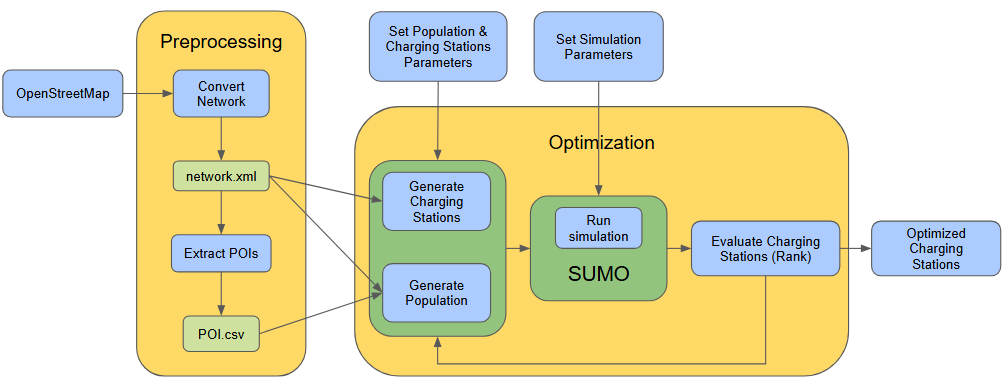
\includegraphics[width=\textwidth]{images/flowchart.png}
    \caption{Flowchart of Creating and Running a Simulation}
    \label{fig:flowchartSUMO}
\end{figure}

As in the previous implementation, an OSM file forms the basis of the entire simulation. This is downloaded using the \texttt{osmGet} tool and serves as the foundation for generating and converting the traffic network (\texttt{network.xml}). In addition, in this implementation, the POIs are extracted directly from the OSM file. Filtering is performed using relevant attributes such as \texttt{amenity="residential", \"office", \"shopping"}, etc., with the results being saved in a CSV file (\texttt{POI.csv}). This step completes the preprocessing state.

The system then generates an initial population and initial distribution of charging stations based on the previously generated files (\texttt{network.xml}, \texttt{POI.csv}) and user-defined parameters. The SUMO simulation can then be started immediately, as no additional conversion steps are required - which is the main advantage of this implementation in comparison to its prototype and significantly reduces the likelihood of errors.

In the subsequent optimization phase, an algorithm works to iteratively improve the placement of charging stations. At the beginning, for example, charging stations are provisionally placed on all road sections (lanes) with a length of more than 70 meters. After a simulation run, the number of vehicles that have charged at each station is recorded. This information is stored in a log file and evaluated. In each iteration, the number of charging stations is then reduced until only a defined targe number of locations remains.

The result of this workflow is an optimized distribution of charging stations based on actual usage, which can be adopted for final deployment.

\subsubsection{Overview of architecture and Dataflow}
As can be seen in the workflow shown above, the implementation comprises three central functionalities:
\begin{itemize}
    \item The generation of trips based on the OSM file and the POI coordinates,
    \item the creation of charging stations on suitable lanes,
    \item and the optimization algorithm for simulation, evaluation and placing the charging stations.
\end{itemize}

These functions are identified in the project structure by the files \texttt{mainGenerateTrips.py}, \texttt{mainGenerateChargingStations.py}, and \texttt{mainSim.py} and are visualized again in the following diagram. The figures also show how the files generated by the first to functions are merged in the simulation.

The three sub-functions are described in detail below.


\begin{figure}[ht]
    \centering
    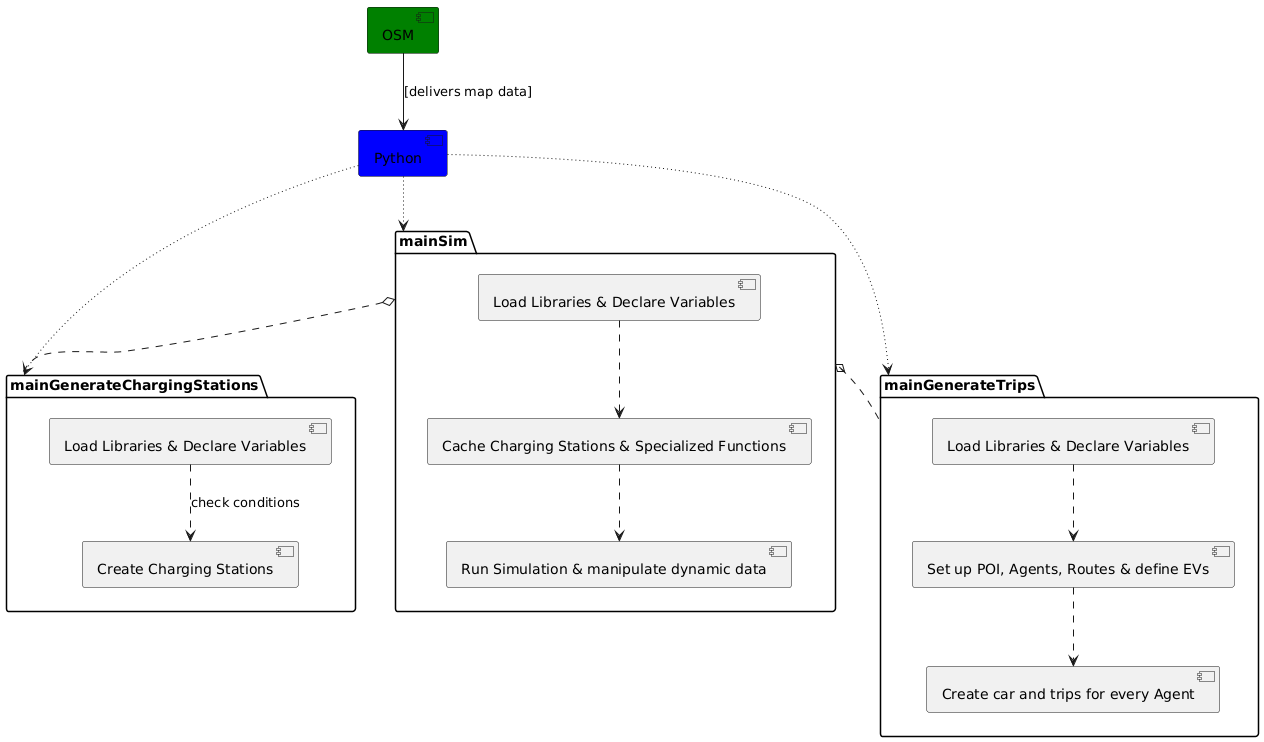
\includegraphics[width=\textwidth]{images/architectureUML.png}
    \caption{Abstracted View of Architecture}
    \label{fig:architecture}
\end{figure}


\subsubsubsection{Population Generation}
The population or trips that the agents follow during simulation are generated automatically from the network and predefined simulation parameters. These include points of interest, the number of desired agents, and the proportion of EVs.

The following activity diagram provides a simplified description of the generation process.
After loading the SUMO network, the edges from the \texttt{POI.csv} that are suitable for car traffic are first validated and filtered. If no edges are valid, the script is aborted to avoid invalid routes.

Then, a loop starts to create agents, i.e., drivers who are to move between POIs on the map. Random home and work edges are selected for each person. In addition, a predetermined proportion is used to decide whether the person will receive an electric vehicle or a conventional vehicle (combustion engine).

In a second loop, an individual vehicle route is created for each person. This includes a random departure time in the morning within the typical rush hour (7-9 a.m.) and an eight-hour stop at the workplace. After route planning, all vehicles are sorted chronologically. The sorting must be done based on the sequential process of SUMO, because it processes each trip one after the other – from top to bottom.

Finally, all vehicles, including their routes and stops, are written to an XML file. Vehicle-specific parameters such as battery capacity and energy behavior are set. The result is a complete file that can be used directly for a SUMO simulation without conversion.

Without this custom script, other frameworks that have already been partially introduced would have to be used to generate the trips, which would increase overhead and the likelihood of errors. With this custom implementation, scenarios can be generated effectively and reliably, completely replacing MATSim.

\begin{figure}[h]
    \centering
    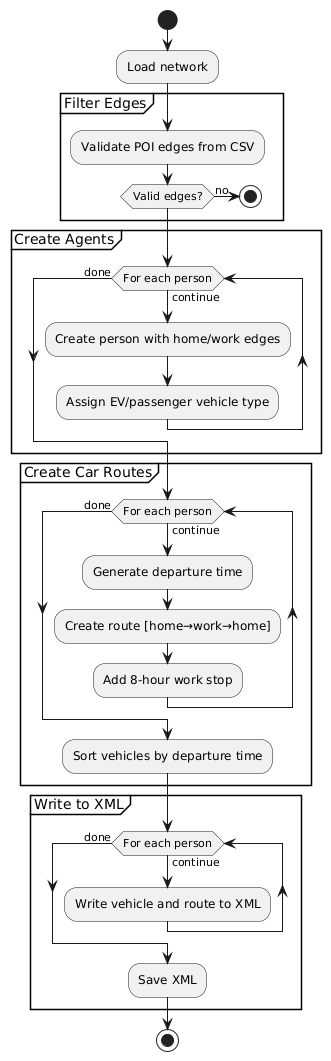
\includegraphics[width=0.32\textwidth]{images/mainTrips_Erik.png}
    \caption{Trip Generation Activity Diagram}
    \label{fig:mainTrips}
\end{figure}

\clearpage
\subsubsubsection{Charging Station Generation}

Just like the trips, the initial charging stations are inserted via a script. The following diagram briefly describes this process.

First, the network is loaded, considering only roads that can actually be used by vehicles. Each of these edges is then validated again. If it fails validation, it is skipped.

Next, all lanes of these valid roads are iterated through. For each lane longer than 70 meters, the center is calculated, a unique ID is generated, and a \texttt{chargingStation} element is created at that location. Each charging station receives fixed values like power capacity and \texttt{chargeInTransit}. The last one restrains cars from charging in active traffic and forces them to park, while doing so.

All generated elements are then used to build an XML structure, which is written to an XML file. This file can be used in the SUMO simulation without any conversion - just like the trips.

It is important to note that these charging stations represent only initial locations, which may be removed during the optimization process by the developed algorithm, for example, if they are not used by EVs.


\begin{figure}[ht]
    \centering
    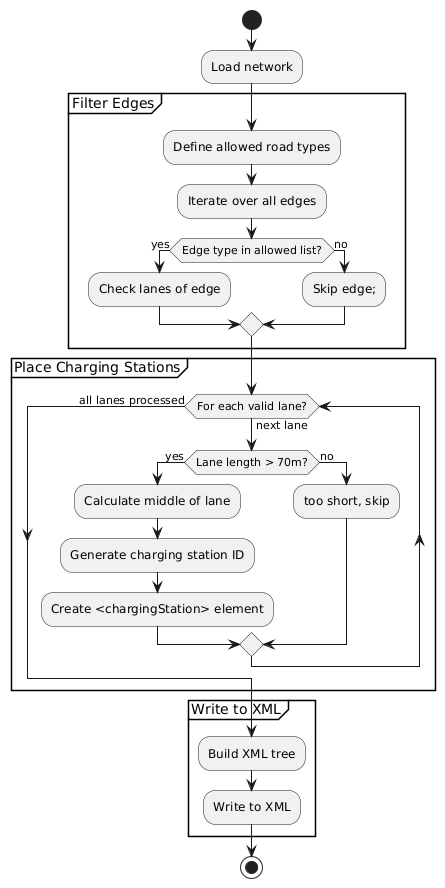
\includegraphics[width=0.41\textwidth]{images/mainChargingStations_Erik.png}
    \caption{Charging Station Deployment Script Activity Diagram}
    \label{fig:mainChargingstation}
\end{figure}

\clearpage
\subsubsubsection{Simulation}
While SUMO acts as the "heart" of the simulation - executing vehicle movements based on preloaded data - TraCI functions as its "brain", providing the ability to dynamically alter the simulations during runtime. Although SUMO could definitely run with only static XML files, TraCI enhances it by allowing real-time control over nearly every simulation aspect. Because of TraCI it is possible to dynamically route and change attributes while using a high level programming logic.

The following activity diagram illustrates an abstracted view of how the simulation is being initialized and how EVs are tracked during the simulation using TraCI.

\begin{figure}[H]
    \centering
    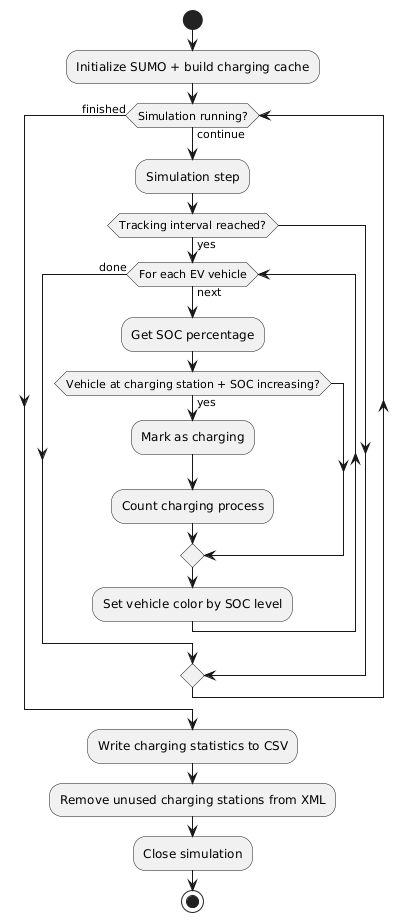
\includegraphics[width=0.43\textwidth]{images/mainSim_Erik.png}
    \caption{System Activity Diagram}
    \label{fig:mainSim}
\end{figure}

At the beginning, the system finally initializes die SUMO simulation - either as GUI or CLI application - and builds a cache of all charging station positions. This cache contains coordinates of all charging stations and improves lookup times during runtime.

Once initialized, the simulation enters its main loop, which continues to run as long as there are active vehicles. Each iteration the simulation advances by one time step.

At specific intervals, which are defined by a tracking interval constant - the system performs deeper analysis. During these intervals, all known EVs are evaluated individually. For each EV, the system retrieves its current state of charge (SOC) in percentage and colors them accordingly.

If a vehicle is found to be stationary at a charging station and its SOC is observed to be increasing, it is marked as actively charging, and the counter for this specific charging station next to it increases. This is important because the optimization algorithm will use it to determine the usage and ranks of the charging stations.

Regardless wether the vehicle is charging, its color is updated based on their SOC level. This visual feedback helps monitoring battery status in real-time within the SUMO-GUI.

Once the simulation loop ends, so all vehicles have left the network (are not active anymore), the system writes a summary of the charging statistics to a CSV file.

\begin{table}[ht]
\centering
\begin{tabular}{|l|c|}
\hline
\rowcolor{gray!20}
\textbf{CS\_id} & \textbf{charges} \\ \hline
CS\_437325054\#0\_0 & 7 \\ \hline
CS\_1100889498\_0   & 4 \\ \hline
CS\_492340367\#1\_0 & 4 \\ \hline
CS\_541295978\#1\_1 & 3 \\ \hline
CS\_437325054\#0\_1 & 1 \\ \hline
CS\_-6228081\#1\_1  & 0 \\ \hline
\end{tabular}
\caption{CS\_id and recorded charges per CS}
\label{tab:cs_charges}
\end{table}

Finally, based on the recorded usage data, the system removes underused or unused charging stations from the XML configuration. The simulation is then properly closed and can be run again in the next iteration.

\begin{table}[ht]
\centering
\begin{tabular}{|l|c|}
\hline
\rowcolor{gray!20}
\textbf{CS\_id} & \textbf{charges} \\ \hline
CS\_437325054\#0\_0 & 7 \\ \hline
CS\_1100889498\_0   & 4 \\ \hline
CS\_492340367\#1\_0 & 4 \\ \hline
\end{tabular}
\caption{CS\_id and recorded charges per CS after removing underused CS stations}
\label{tab:cs_charges2}
\end{table}

This workflow enables dynamic tracking of EV charging behavior and allows post-simulation filtering of charging infrastructure. It can be repeated as long as the user wishes for or the number of charging stations doesn't decrease anymore.


